\documentclass[10pt]{beamer}
\usetheme{metropolis}
% all imports
\usepackage[utf8]{inputenc}
\usepackage{lmodern}
\usepackage[T1]{fontenc}
\usepackage{appendixnumberbeamer}
\usepackage{hyperref}
\usepackage{booktabs}
\usepackage{bm}
\usepackage[scale=2]{ccicons}
\usepackage[cache=false]{minted}
\usepackage{pgfplots}
\usepackage{array,colortbl,xcolor}
\usepgfplotslibrary{dateplot}
\usepackage{setspace}
\usepackage{etoolbox}
\usepackage{xspace}
\usepackage{tikz}
\usetikzlibrary{shapes,arrows,positioning,fit,backgrounds}
\usepackage{tkz-euclide}

\AtBeginEnvironment{quote}{\singlespacing}


\AtBeginEnvironment{quote}{\singlespacing}

% new commands
\input{all_new_commands}

% definitions
\input{definitions/colors}
% Tikzstyles for Computation Graphs

% nodes
\tikzstyle{noop} = [circle, draw=none, fill=red, minimum size = 10pt]
\tikzstyle{op} = [circle, draw=red, line width=1.5pt, fill=red!70, text=black,
text centered, font=\bf \normalsize, minimum size = 15pt]
\tikzstyle{state} = [circle, draw=blue, line width=1.5pt, fill=blue!70, text=black, text centered, font=\bf \normalsize, minimum size = 25pt]
% \tikzstyle{gradient} = [circle, draw=green, line width=1.5pt, fill=green!60, text=black, text centered, font=\bf \normalsize, minimum size = 25pt]
\tikzstyle{gradient} = [circle, draw=nephritis, line width=1.5pt, fill=nephritis!60, text=black, text centered, font=\bf \normalsize, minimum size = 25pt]
\tikzstyle{textonly} = [draw=none, fill=none, text centered, font=\bf \normalsize]
\tikzstyle{rectangle}= [draw=green, line width=1.5pt, fill=green!70, text=black,
text centered, font=\bf \normalsize, minimum size = 25pt]
\tikzstyle{block} = [rectangle, draw, fill=red!40,
text width=6em, text centered, rounded corners, minimum height=3em]

% edges
% \tikzstyle{tedge}  = [draw, thick, >=stealth, ->]
\tikzstyle{tedge}  = [draw, thick, >=latex, ->]
\tikzstyle{tedge_dashed}  = [draw, thick, >=latex, ->, dashed]

% namedscope
\tikzstyle{namedscope} = [circle, draw=orange, line width=1.5pt, fill=orange!60, align=center, inner sep=0pt]

% \tikzstyle{container} = [draw=none, rectangle, dotted, inner ysep=1.5em]
% \tikzstyle{novertex} = [draw=none, fill=none, text centered]
% \tikzstyle{predicate} = [ellipse, draw, thick, text centered, rounded corners, minimum size=30pt]
% \tikzstyle{aux} = [rectangle, draw, thick, text centered, rounded corners, minimum size=30pt]
% \tikzstyle{ledge}  = [draw, dashed, thick, >=stealth, ->]
% \tikzstyle{pedge}  = [draw, thick, >=stealth, ->]



\title{Deep Active Learning for sentiment analysis}
\date{\today}

\author{
  Lucas Moura\\
  \url{https://github.com/lucasmoura}
  \vspace{0.4 cm}
}

\institute{\textbf{IME-USP}: Institute of Mathematics and Statistics, University of São Paulo}


\begin{document}

\maketitle

\section{Introduction}

\begin{frame}[fragile]{Motivation}
\begin{itemize}
\item \alert{Deep Learning} is a growing field with state-of-the-art result in
    several areas.
\vspace{0.5cm}
\item Image Classification, Natural Language Processing
\end{itemize}
\end{frame}

\begin{frame}[fragile]
    \begin{figure}[htp]
        \centering
        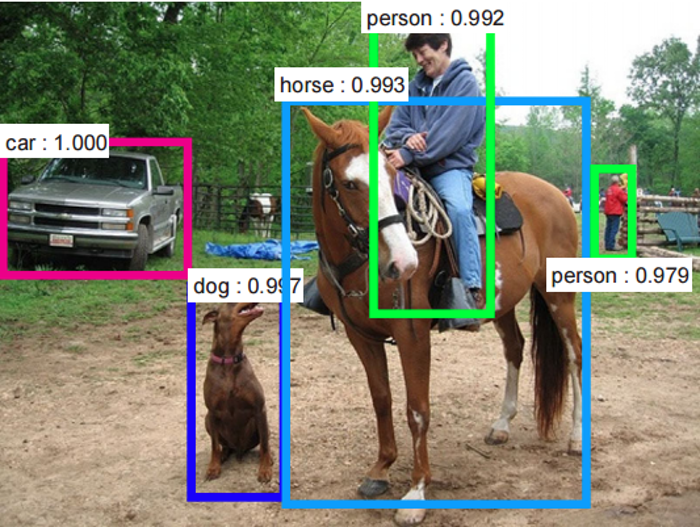
\includegraphics[scale=0.4]{images/image_classification.png}
        \caption{Image recognition by Deep Learning model \cite{faster_r_cnn}}
    \end{figure}
\end{frame}

\section{However...}

\begin{frame}[fragile]
\begin{itemize}
\item Training \alert{Deep Learning} models require a huge amount of labeled data
\vspace{0.5cm}
\item For the task of image classification on the ImageNet database, 1.2 million
    labeled images were used \cite{imagenet}
\end{itemize}
\end{frame}

\begin{frame}[fragile]{Sentiment Analysis}
\begin{itemize}
\item Verify if a text is expressing negative or positive feelings.
\vspace{0.5cm}
\item Huge amount of data, but few labeled.
\end{itemize}
\end{frame}

\section{Active Learning}

\begin{frame}[fragile]{Active Learning}
    \begin{figure}[htp]
        \centering
        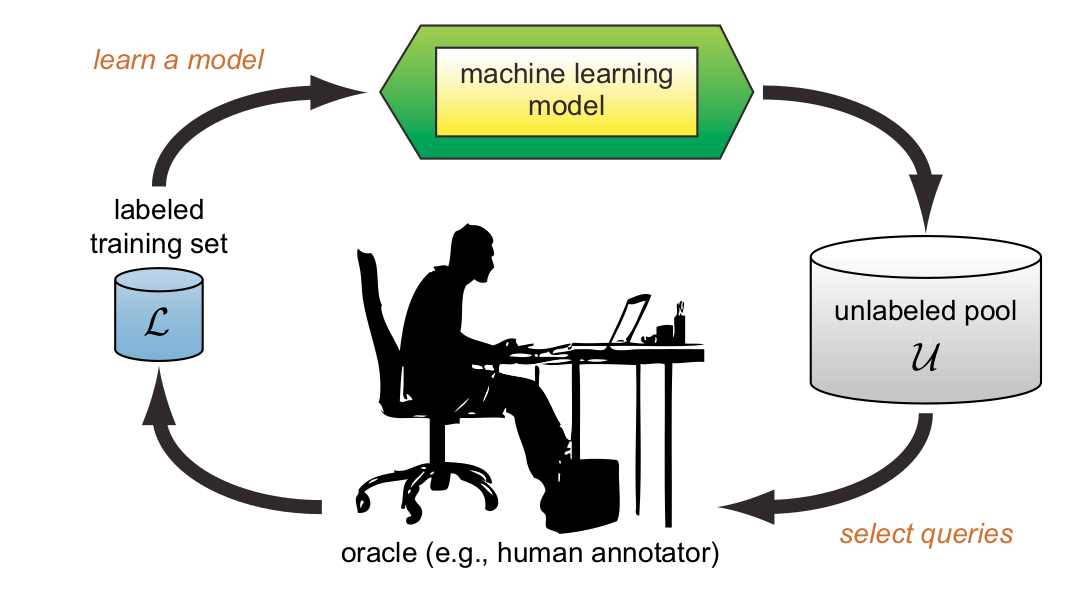
\includegraphics[scale=0.3]{images/active_learning.png}
        \caption{Active Learning cycle \cite{active_learning}}
    \end{figure}
\end{frame}

\begin{frame}[fragile]{Active Learning}
    \begin{figure}[htp]
        \centering
        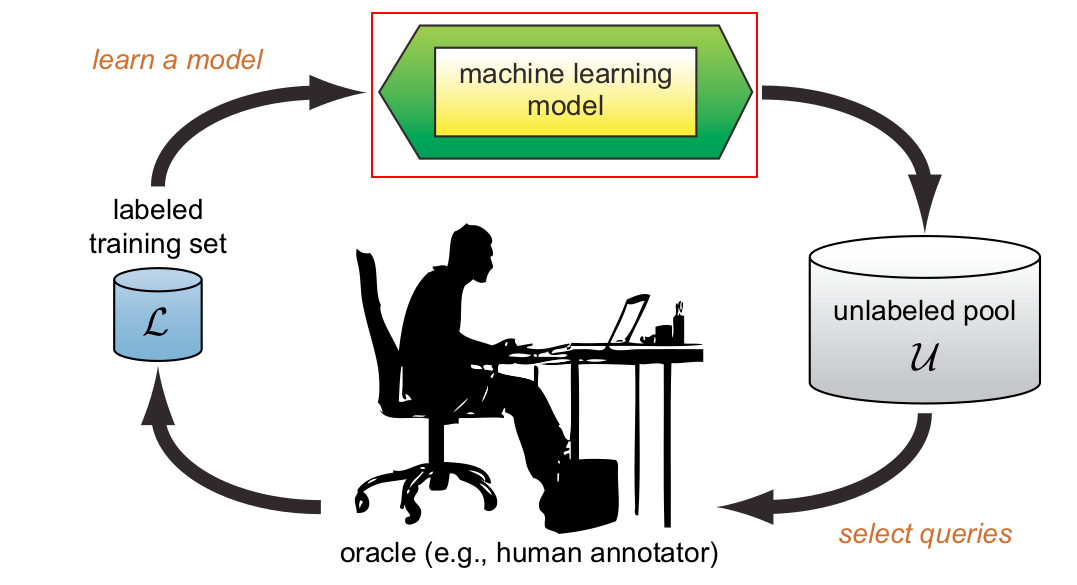
\includegraphics[scale=0.3]{images/active_learning_ml_model.png}
    \end{figure}
\end{frame}

\begin{frame}[fragile]{Active Learning}
    \begin{figure}[htp]
        \centering
        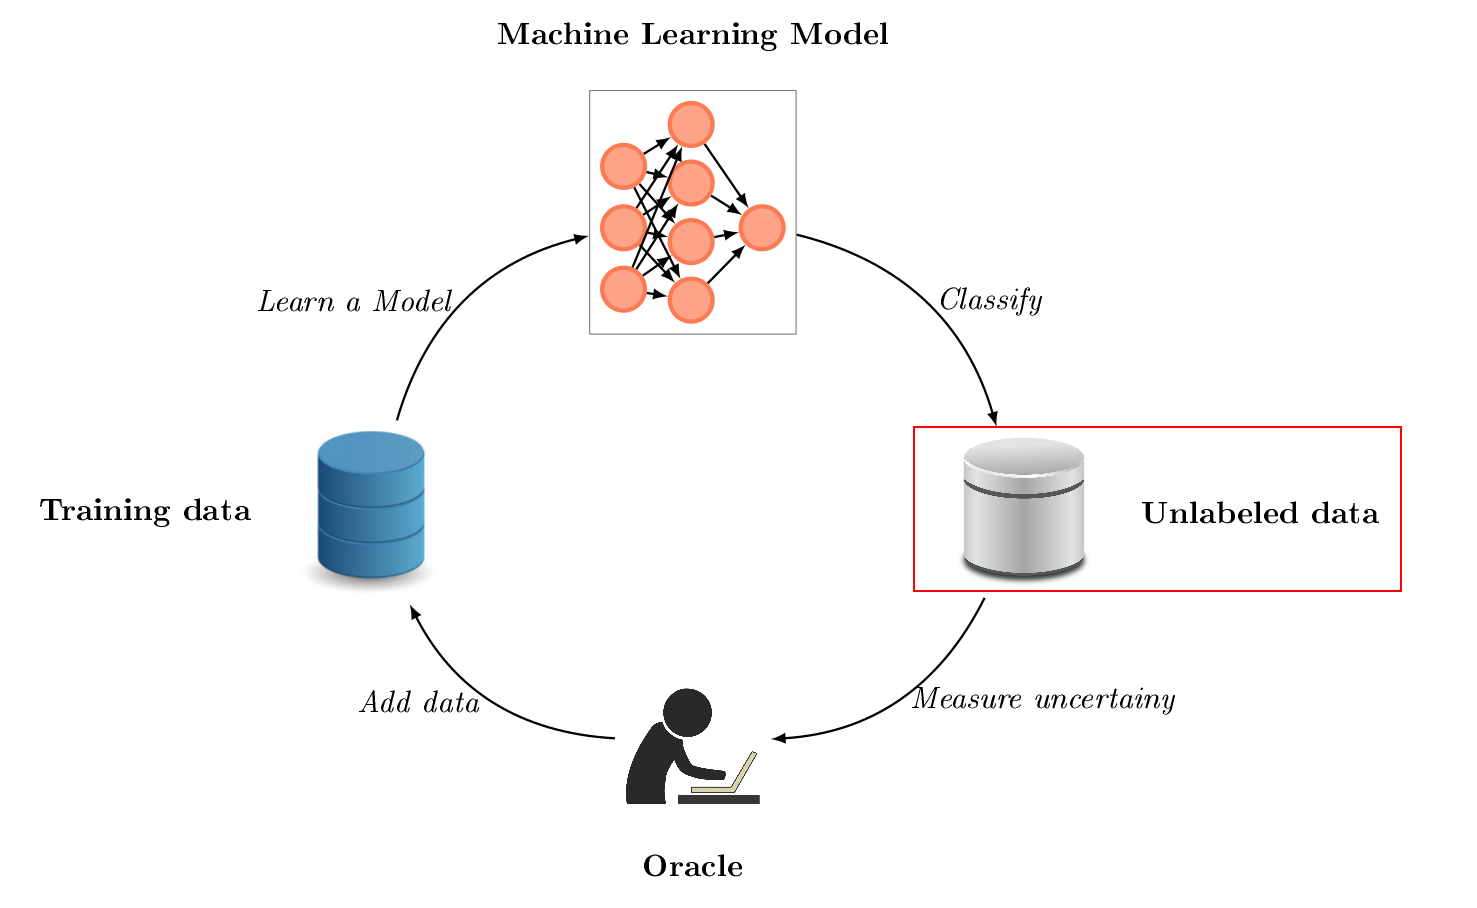
\includegraphics[scale=0.3]{images/active_learning_unlabeled.png}
    \end{figure}
\end{frame}

\begin{frame}[fragile]{Active Learning}
    \begin{figure}[htp]
        \centering
        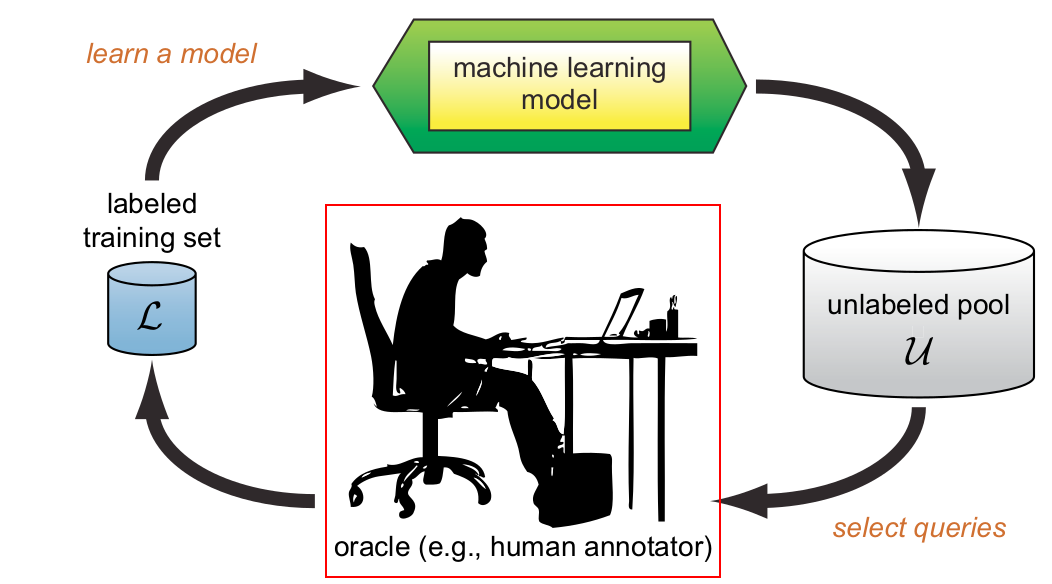
\includegraphics[scale=0.3]{images/active_learning_oracle.png}
    \end{figure}
\end{frame}

\begin{frame}[fragile]{Active Learning}
    \begin{figure}[htp]
        \centering
        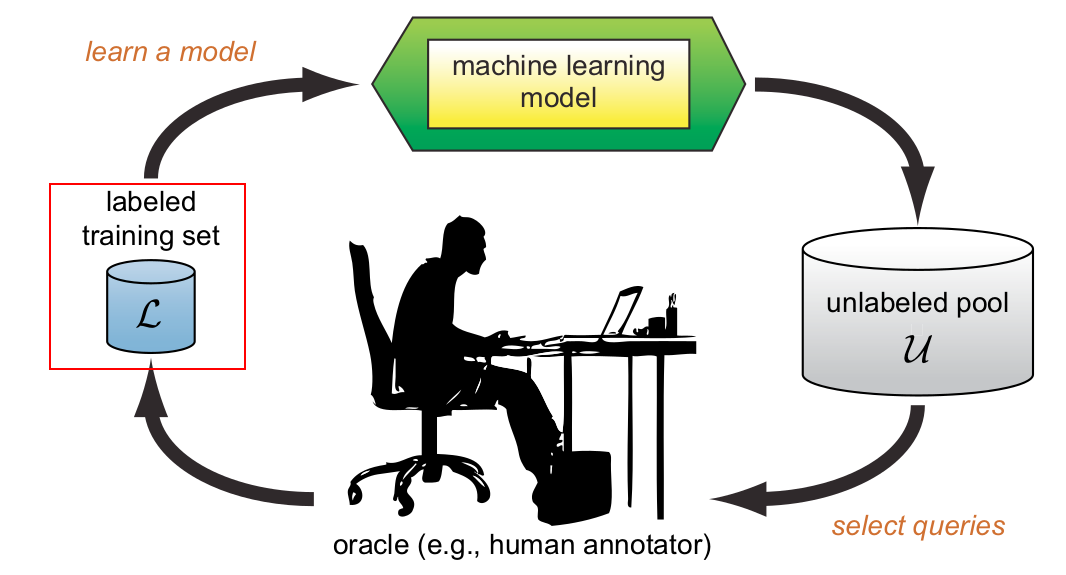
\includegraphics[scale=0.3]{images/active_learning_labeled.png}
    \end{figure}
\end{frame}

\begin{frame}[fragile]{Active Learning}
    \begin{figure}[htp]
        \centering
        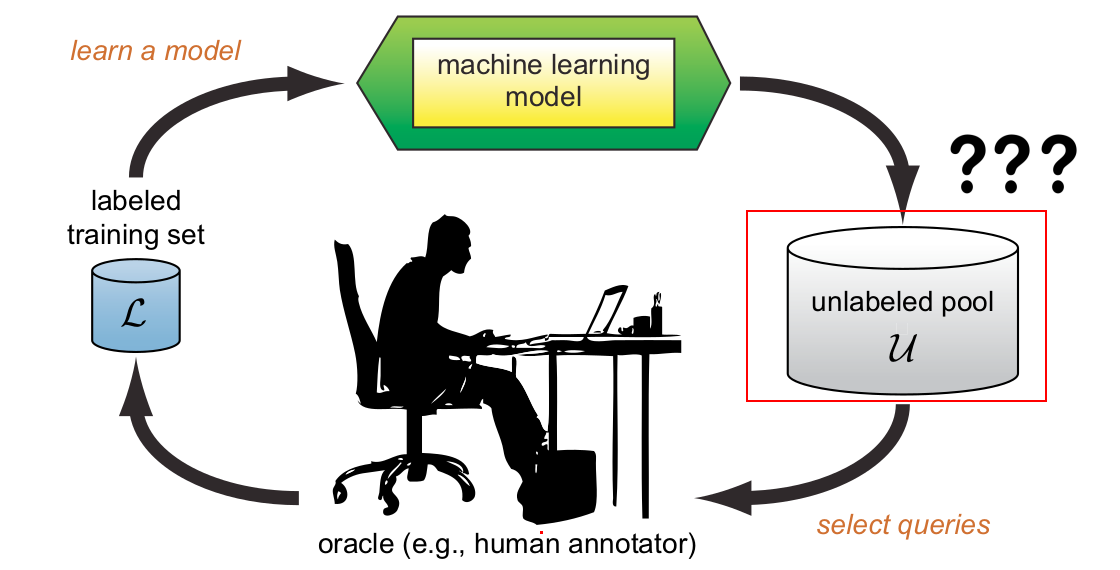
\includegraphics[scale=0.3]{images/active_learning_uncertainty.png}
    \end{figure}
\end{frame}

\begin{frame}[fragile]{Neural Network}
    \begin{figure}[ht!]
\centering

\scalebox{1.0}{
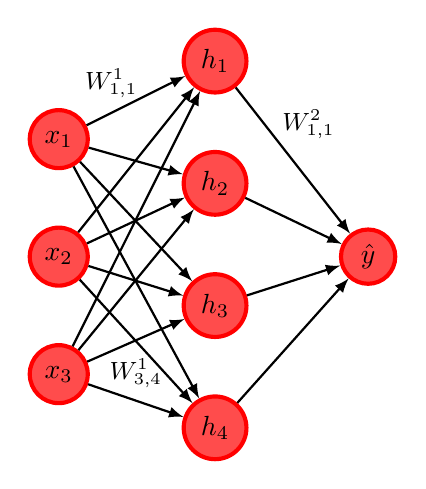
\begin{tikzpicture}[auto]

% operations =============================
\node[op] (x2) {$x_2$};
\node[op, above=20pt of x2] (x1) {$x_1$};
\node[op, below=20pt of x2] (x3) {$x_3$};
\node[op, above right=10pt and 40pt of x2] (h2) {$h_2$};
\node[op, above=20pt of h2] (h1) {$h_1$};
\node[op, below=20pt of h2] (h3) {$h_3$};
\node[op, below=20pt of h3] (h4) {$h_4$};
\node[op, right=90pt of x2] (y) {$\hat{y}$};

% edges
\path[tedge] (x1) edge node[pos=0.25, above=1.8pt] {\alert{\small $\vect{W}_{1,1}^{1}$}} (h1);
\path[tedge] (x1) edge node[above=1.2pt] {} (h2);
\path[tedge] (x1) edge node[above=1.8pt] {} (h3);
\path[tedge] (x1) edge node[above=1.8pt] {} (h4);

\path[tedge] (x2) edge node[above=1.8pt] {} (h1);
\path[tedge] (x2) edge node[above=1.8pt] {} (h2);
\path[tedge] (x2) edge node[above=1.8pt] {} (h3);
\path[tedge] (x2) edge node[above=1.8pt] {} (h4);

\path[tedge] (x3) edge node[above=1.8pt] {} (h1);
\path[tedge] (x3) edge node[above=1.8pt] {} (h2);
\path[tedge] (x3) edge node[above=1.8pt] {} (h3);
\path[tedge] (x3) edge node[above=1.0pt] {\small $\vect{W}_{3,4}^{1}$} (h4);

\path[tedge] (h1) edge node[pos=0.25, above=1.8pt, right=0.1cm] {\small $\vect{W}_{1,1}^{2}$} (y);
\path[tedge] (h2) edge node[above=1.8pt] {} (y);
\path[tedge] (h3) edge node[above=1.8pt] {} (y);
\path[tedge] (h4) edge node[above=1.8pt] {} (y);

% info edges


\end{tikzpicture}
} % scalebox
\end{figure}

\end{frame}

\begin{frame}[fragile]{Bayesian Neural Network}
    \begin{figure}[htp]
        \centering
        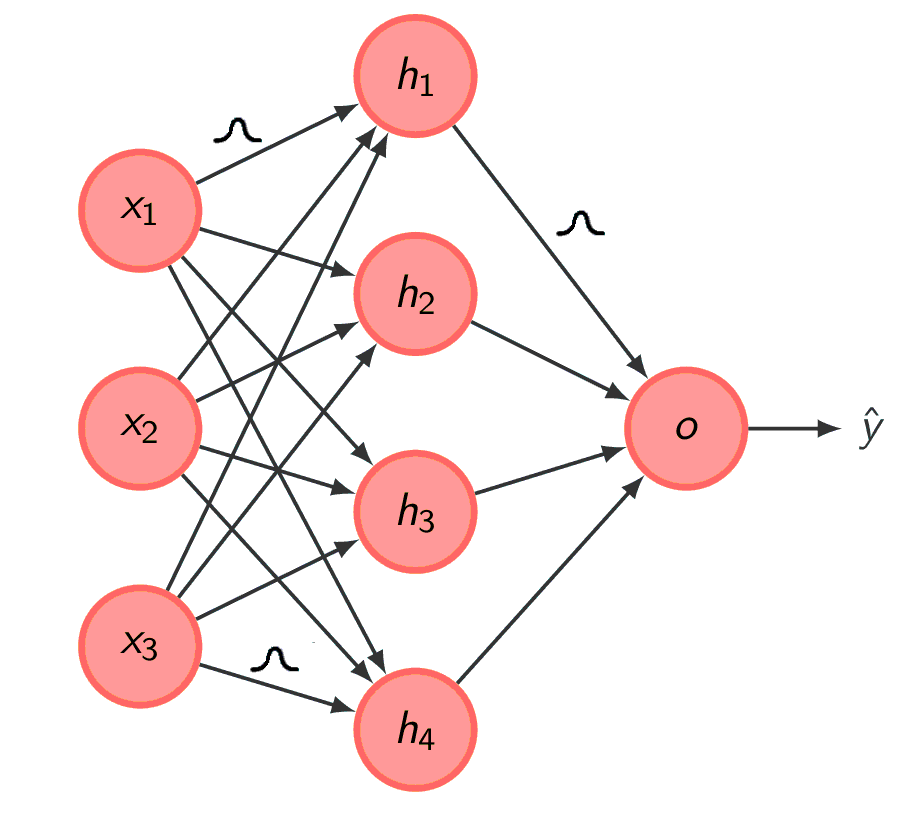
\includegraphics[scale=0.3]{images/bayesian_neural_network.png}
    \end{figure}
\end{frame}

\begin{frame}[fragile]{Bayesian Neural Network}
    \begin{figure}[ht!]
\centering

\scalebox{1.2}{
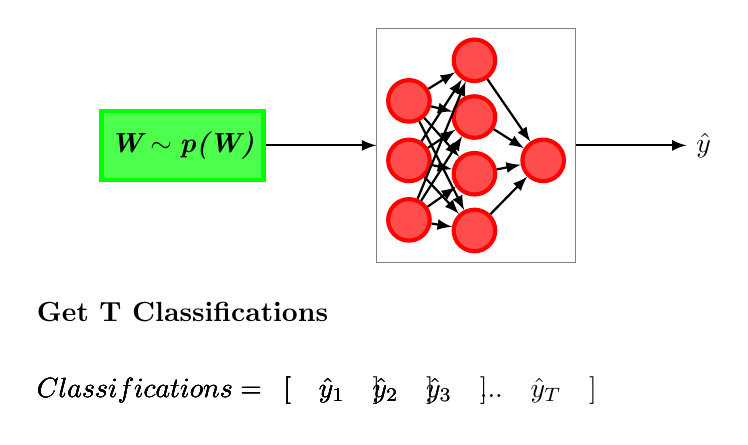
\begin{tikzpicture}[auto]

% operations =============================

\visible<2->{
\node[op] (x2) {};
\node[op, above=5pt of x2] (x1) {};
\node[op, below=5pt of x2] (x3) {};
\node[op, above right=4pt and 12pt of x2] (h2) {};
\node[op, above=4pt of h2] (h1) {};
\node[op, below=4pt of h2] (h3) {};
\node[op, below=4pt of h3] (h4) {};
\node[op, right=32pt of x2] (o) {};

% edges
\path[tedge] (x1) edge node[pos=0.25, above=1.8pt] {} (h1);
\path[tedge] (x1) edge node[above=1.2pt] {} (h2);
\path[tedge] (x1) edge node[above=1.8pt] {} (h3);
\path[tedge] (x1) edge node[above=1.8pt] {} (h4);

\path[tedge] (x2) edge node[above=1.8pt] {} (h1);
\path[tedge] (x2) edge node[above=1.8pt] {} (h2);
\path[tedge] (x2) edge node[above=1.8pt] {} (h3);
\path[tedge] (x2) edge node[above=1.8pt] {} (h4);

\path[tedge] (x3) edge node[above=1.8pt] {} (h1);
\path[tedge] (x3) edge node[above=1.8pt] {} (h2);
\path[tedge] (x3) edge node[above=1.8pt] {} (h3);
\path[tedge] (x3) edge node[above=1.0pt] {} (h4);

\path[tedge] (h1) edge node[pos=0.25, above=1.8pt, right=0.1cm] {} (o);
\path[tedge] (h2) edge node[above=1.8pt] {} (o);
\path[tedge] (h3) edge node[above=1.8pt] {} (o);
\path[tedge] (h4) edge node[above=1.8pt] {} (o);

\node [draw=black!50, fit={(x1) (x2) (x3) (h1) (h2) (h3) (h4) (o)}] (nn) {};
% edges
}

\node[rectangle, left=40pt of nn] (w) {$\textit{W} \sim \textit{p(W)}$};

\visible<2->{
  \path[tedge] (w) edge node[above=1.8pt] {} (nn);
}

\visible<3->{
\node[textonly, right=40pt of nn] (y) {$\hat{y}$};
\path[tedge] (nn) edge node[above=1.8pt] {} (y);
}

\visible<4->{
\node[textonly, below=40pt of w] (t_text) {Get T Classifications};
}

\visible<5>{
\node[textonly, right, below=of t_text.west,anchor=west] (a1) {$
  Classifications = \begin{array}{ccc}[& \hat{y}_{1} & ]\end{array}
$};
}

\visible<6>{
\node[textonly, below=of t_text.west,anchor=west] (a1) {$
  Classifications = \begin{array}{cccc}[& \hat{y}_{1} & \hat{y}_{2} & ]\end{array}
$};
}

\visible<7>{
\node[textonly, below=of t_text.west,anchor=west] (a1) {$
  Classifications = \begin{array}{ccccc}[& \hat{y}_{1} & \hat{y}_{2} &
  \hat{y}_{3} & ]\end{array}
$};
}

\visible<8>{
\node[textonly, below=of t_text.west,anchor=west] (a1) {$
Classifications = \begin{array}{ccccccc}[& \hat{y}_{1} & \hat{y}_{2} &
\hat{y}_{3} & ... & \hat{y}_{T} & ]\end{array}
$};
}

\end{tikzpicture}
} % scalebox
\end{figure}

\end{frame}

\begin{frame}[fragile]{Bayesian Neural Network}
\begin{itemize}
\item Train such network is a costly process
\vspace{0.5cm}
\item Use techniques such as variational inference and Monte Carlo Estimation
\end{itemize}
\end{frame}

\begin{frame}[fragile]{Bayesian Neural Network}
\begin{itemize}
\item What if we could extract uncertainty measurements from current Deep
    Learning models if they use stachastic regularization techniques such as
        \alert{Dropout} ?
\vspace{0.5cm}
\item Uncertainty in Deep Learning (Yarin Gal, 2017)
\end{itemize}
\end{frame}

\section{Dropout}

\begin{frame}[fragile]{Dropout}
\begin{itemize}
\item During training some weights are dropped from the network
\end{itemize}
\end{frame}

\begin{frame}[fragile]{Dropout}
    \begin{figure}[ht!]
\centering

\scalebox{1.0}{
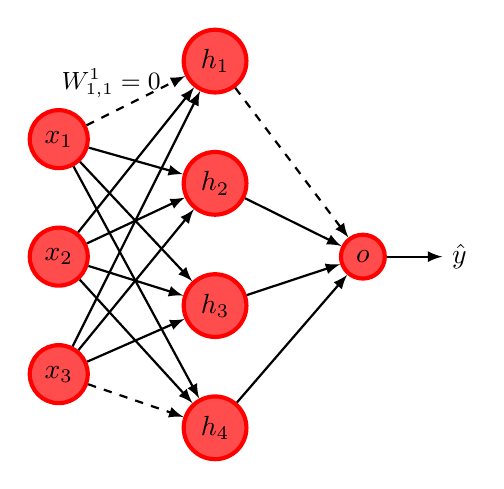
\begin{tikzpicture}[auto]

% operations =============================
\node[op] (x2) {$x_2$};
\node[op, above=20pt of x2] (x1) {$x_1$};
\node[op, below=20pt of x2] (x3) {$x_3$};
\node[op, above right=10pt and 40pt of x2] (h2) {$h_2$};
\node[op, above=20pt of h2] (h1) {$h_1$};
\node[op, below=20pt of h2] (h3) {$h_3$};
\node[op, below=20pt of h3] (h4) {$h_4$};
\node[op, right=90pt of x2] (o) {$o$};
\node[textonly, right=20pt of o] (y) {$\hat{y}$};

% edges
\path[tedge_dashed] (x1) edge node[pos=0.25, above=1.8pt, dashed] {
  \small $\vect{W}_{1,1}^{1} = 0$} (h1);
\path[tedge] (x1) edge node[above=1.2pt] {} (h2);
\path[tedge] (x1) edge node[above=1.8pt] {} (h3);
\path[tedge] (x1) edge node[above=1.8pt] {} (h4);

\path[tedge] (x2) edge node[above=1.8pt] {} (h1);
\path[tedge] (x2) edge node[above=1.8pt] {} (h2);
\path[tedge] (x2) edge node[above=1.8pt] {} (h3);
\path[tedge] (x2) edge node[above=1.8pt] {} (h4);

\path[tedge] (x3) edge node[above=1.8pt] {} (h1);
\path[tedge] (x3) edge node[above=1.8pt] {} (h2);
\path[tedge] (x3) edge node[above=1.8pt] {} (h3);
\path[tedge_dashed] (x3) edge node[above=1.0pt] {} (h4);

\path[tedge_dashed] (h1) edge node[pos=0.25, above=1.8pt, right=0.1cm] {} (o);
\path[tedge] (h2) edge node[above=1.8pt] {} (o);
\path[tedge] (h3) edge node[above=1.8pt] {} (o);
\path[tedge] (h4) edge node[above=1.8pt] {} (o);

\path[tedge] (o) edge node[above=1.8pt] {} (y);

% info edges


\end{tikzpicture}
} % scalebox
\end{figure}

\end{frame}

\begin{frame}[fragile]{Dropout}
    \begin{figure}[ht!]
\centering

\scalebox{1.0}{
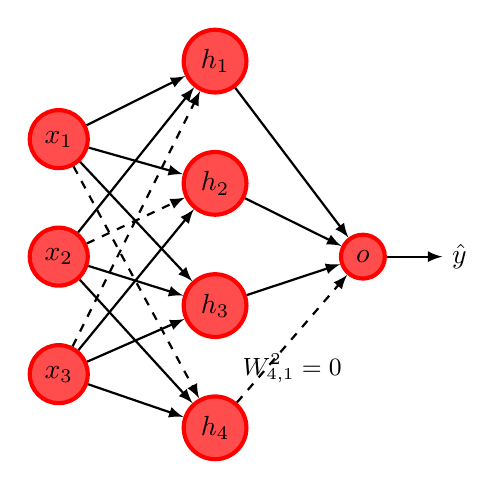
\begin{tikzpicture}[auto]

% operations =============================
\node[op] (x2) {$x_2$};
\node[op, above=20pt of x2] (x1) {$x_1$};
\node[op, below=20pt of x2] (x3) {$x_3$};
\node[op, above right=10pt and 40pt of x2] (h2) {$h_2$};
\node[op, above=20pt of h2] (h1) {$h_1$};
\node[op, below=20pt of h2] (h3) {$h_3$};
\node[op, below=20pt of h3] (h4) {$h_4$};
\node[op, right=90pt of x2] (o) {$o$};
\node[textonly, right=20pt of o] (y) {$\hat{y}$};

% edges
\path[tedge] (x1) edge node[pos=0.25, above=1.8pt] {} (h1);
\path[tedge] (x1) edge node[above=1.2pt] {} (h2);
\path[tedge] (x1) edge node[above=1.8pt] {} (h3);
\path[tedge_dashed] (x1) edge node[above=1.8pt] {} (h4);

\path[tedge] (x2) edge node[above=1.8pt] {} (h1);
\path[tedge_dashed] (x2) edge node[above=1.8pt] {} (h2);
\path[tedge] (x2) edge node[above=1.8pt] {} (h3);
\path[tedge] (x2) edge node[above=1.8pt] {} (h4);

\path[tedge_dashed] (x3) edge node[above=1.8pt] {} (h1);
\path[tedge] (x3) edge node[above=1.8pt] {} (h2);
\path[tedge] (x3) edge node[above=1.8pt] {} (h3);
\path[tedge] (x3) edge node[above=1.0pt] {} (h4);

\path[tedge] (h1) edge node[pos=0.25, above=1.8pt, right=0.1cm] {} (o);
\path[tedge] (h2) edge node[above=1.8pt] {} (o);
\path[tedge] (h3) edge node[above=1.8pt] {} (o);
\path[tedge_dashed] (h4) edge node[below=1.8pt] {\small $\vect{W}_{4,1}^{2} = 0$}(o);

\path[tedge] (o) edge node[above=1.8pt] {} (y);

% info edges


\end{tikzpicture}
} % scalebox
\end{figure}

\end{frame}

\begin{frame}[fragile]{Dropout}
\begin{itemize}
    \item The optimization of Neural Network using \alert{Dropout} is practicaly the same
        as the optimization function of a Network trained with \alert{Variational
        Inference}.
    \vspace{0.5cm}
    \item Therefore it is possible to extract uncertainty measures from these
        networks.
\end{itemize}
\end{frame}

\begin{frame}[fragile]{Bayesian Neural Network}
    \begin{figure}[ht!]
\centering

\scalebox{1.0}{
\begin{tikzpicture}[auto]

% operations =============================

\visible<3->{
\node[op] (x2) {};
\node[op, above=5pt of x2] (x1) {};
\node[op, below=5pt of x2] (x3) {};
\node[op, above right=4pt and 16pt of x2] (h2) {};
\node[op, above=4pt of h2] (h1) {};
\node[op, below=4pt of h2] (h3) {};
\node[op, below=4pt of h3] (h4) {};
\node[op, right=32pt of x2] (o) {};

% edges
\path[tedge] (x1) edge node[pos=0.25, above=1.8pt] {} (h1);
\path[tedge] (x1) edge node[above=1.2pt] {} (h2);
\path[tedge] (x1) edge node[above=1.8pt] {} (h3);
\path[tedge] (x1) edge node[above=1.8pt] {} (h4);

\path[tedge] (x2) edge node[above=1.8pt] {} (h1);
\path[tedge_dashed] (x2) edge node[above=1.8pt] {} (h2);
\path[tedge] (x2) edge node[above=1.8pt] {} (h3);
\path[tedge] (x2) edge node[above=1.8pt] {} (h4);

\path[tedge] (x3) edge node[above=1.8pt] {} (h1);
\path[tedge] (x3) edge node[above=1.8pt] {} (h2);
\path[tedge_dashed] (x3) edge node[above=1.8pt] {} (h3);
\path[tedge] (x3) edge node[above=1.0pt] {} (h4);

\path[tedge_dashed] (h1) edge node[pos=0.25, above=1.8pt, right=0.1cm] {} (o);
\path[tedge] (h2) edge node[above=1.8pt] {} (o);
\path[tedge] (h3) edge node[above=1.8pt] {} (o);
\path[tedge] (h4) edge node[above=1.8pt] {} (o);

\node [draw=black!50, fit={(x1) (x2) (x3) (h1) (h2) (h3) (h4) (o)}] (nn) {};

% edges
\path[tedge] (w) edge node[above=1.8pt] {} (nn);
}

\node[rectangle, left=40pt of nn] (w) {\small$\textit{E} \sim \textit{Bernoulli}$};

\visible<2->{
\node[textonly, above=20pt of w] (e) {\small$
   Dropout = \begin{array}{cccccc}[& 0 & 1 & ... & 0 & ]\end{array} $};
\path[tedge] (w) edge node[above=1.8pt] {} (e);
}

\visible<4->{
\node[textonly, right=40pt of nn] (y) {$\hat{y}$};
\path[tedge] (nn) edge node[above=1.8pt] {} (y);
}

\visible<5->{
\node[textonly, below=40pt of w] (t_text) {Get T Classifications};
}

\visible<6>{
\node[textonly, right, below=of t_text.west,anchor=west] (a1) {$
  Classifications = \begin{array}{ccc}[& \hat{y}_{1} & ]\end{array}
$};
}

\visible<7>{
\node[textonly, below=of t_text.west,anchor=west] (a1) {$
  Classifications = \begin{array}{cccc}[& \hat{y}_{1} & \hat{y}_{2} & ]\end{array}
$};
}

\visible<8>{
\node[textonly, below=of t_text.west,anchor=west] (a1) {$
  Classifications = \begin{array}{ccccc}[& \hat{y}_{1} & \hat{y}_{2} &
  \hat{y}_{3} & ]\end{array}
$};
}

\visible<9>{
\node[textonly, below=of t_text.west,anchor=west] (a1) {$
Classifications = \begin{array}{ccccccc}[& \hat{y}_{1} & \hat{y}_{2} &
\hat{y}_{3} & ... & \hat{y}_{T} & ]\end{array}
$};
}

\end{tikzpicture}
} % scalebox
\end{figure}

\end{frame}

\begin{frame}[fragile]{What's next}
\begin{itemize}
    \item Use this uncertainty measure to perform active learning together with
        sentiment analysis.
    \vspace{0.5cm}
    \item Choose which Deep Learning model to use for sentiment analysis (probably
        LSTM)
    \vspace{0.5cm}
    \item Choose which selection metrics are normally used for text analysis
        together with active learning.
\end{itemize}
\end{frame}

\begin{frame}[allowframebreaks]{References}
  \bibliography{demo}
  \bibliographystyle{abbrv}
\end{frame}

\end{document}
